\documentclass[conference]{IEEEtran}
\IEEEoverridecommandlockouts
% The preceding line is only needed to identify funding in the first footnote. If that is unneeded, please comment it out.

\usepackage{listings}
\usepackage{lipsum}
\usepackage{float} 
\usepackage{caption}
\usepackage{subcaption}
\usepackage{graphicx}
%\usepackage{hyperref}
\usepackage{multirow}
\usepackage[table]{xcolor}
\usepackage{graphicx}
\graphicspath{ {imagenes/} }
\usepackage{enumitem}
\usepackage{tabularx}
\usepackage{xcolor}


%\usepackage[round,sort,numbers,authoryear]{natbib}
%\usepackage{usebib}
%\bibpunct{[}{]}{;}{n}{,}{,}

% *** CITATION PACKAGES ***
%
\ifCLASSOPTIONcompsoc
  % IEEE Computer Society needs nocompress option
  % requires cite.sty v4.0 or later (November 2003)
  \usepackage[nocompress]{cite}
\else
  % normal IEEE
  \usepackage{cite}
\fi


%
\ifCLASSINFOpdf
  % \usepackage[pdftex]{graphicx}
  % declare the path(s) where your graphic files are
  % \graphicspath{{../pdf/}{../jpeg/}}
  % and their extensions so you won't have to specify these with
  % every instance of \includegraphics
  % \DeclareGraphicsExtensions{.pdf,.jpeg,.png}
\else
  % or other class option (dvipsone, dvipdf, if not using dvips). graphicx
  % will default to the driver specified in the system graphics.cfg if no
  % driver is specified.
  % \usepackage[dvips]{graphicx}
  % declare the path(s) where your graphic files are
  % \graphicspath{{../eps/}}
  % and their extensions so you won't have to specify these with
  % every instance of \includegraphics
  % \DeclareGraphicsExtensions{.eps}
\fi



% correct bad hyphenation here
\hyphenation{op-tical net-works semi-conduc-tor}

\makeatletter
\newcommand{\linebreakand}{%
  \end{@IEEEauthorhalign}
  \hfill\mbox{}\par
  \mbox{}\hfill\begin{@IEEEauthorhalign}
}
\makeatother

\begin{document}
%
% paper title
% Titles are generally capitalized except for words such as a, an, and, as,
% at, but, by, for, in, nor, of, on, or, the, to and up, which are usually
% not capitalized unless they are the first or last word of the title.
% Linebreaks \\ can be used within to get better formatting as desired.
% Do not put math or special symbols in the title.
\title{Estimation of Object Location in Small Enclosed Spaces Using Convolucional Neural Network and Acoustic Echoes}


% author names and affiliations
% use a multiple column layout for up to three different
% affiliations
\author{
\IEEEauthorblockN{Esteban Padilla Padilla}
\IEEEauthorblockA{\textit{Instituto Tecnológico de Costa Rica}\\
San José, Costa Rica\\
estebanpadi@estudiantec.cr}
\and
\IEEEauthorblockN{Kervin Sánchez Herrera}
\IEEEauthorblockA{\textit{Instituto Tecnológico de Costa Rica}\\
San José, Costa Rica\\
ksanchez@itcr.ac.cr}

}


\maketitle

\begin{abstract}
 Robotic perception must excel when machines are deployed to operate and interact safely with humans in complex environments. Acoustic perception of geometries and enclosed spaces represents a promising modality to complement and enhance traditional optical sensing. This work investigates the use of acoustic sensing and Convolutional Neural Networks (CNNs) to estimate the spatial location of an object inside a confined environment. An experimental measurement box was constructed, equipped with a robotic arm to position a cube at controlled coordinates and orientations, and instrumented with a speaker and a four‑microphone array to capture the acoustic response. A dataset of acoustic recordings was collected covering a wide range of cube positions and orientations per location. Spectrograms were generated from the audio signals and used as input to a modified ResNet‑18 architecture designed for both classification and regression tasks.
The model achieved high accuracy in classifying cube location regions, while orientation classification proved significantly more challenging.
For coordinate estimation, three independent regression networks were trained to predict the X, Y, and Z positions of the cube, for each coordinate the estimation error is presented and analyzed. Overall, the findings demonstrate that acoustic perception combined with CNN‑based inference can effectively estimate the location of objects in reduced spaces, offering a low‑cost alternative to optical sensors. 

\end{abstract}   

\begin{IEEEkeywords}
Audio, Room Impulse Response, CNN, Log-Mel spectrogram, location estimation.
\end{IEEEkeywords}


\IEEEpeerreviewmaketitle

\section{Introduction}

Robots are expected to operate across multiple and diverse environments. To achieve this, they must be endowed with situational awareness and sufficient autonomy to make appropriate decisions. Computer vision seeks to provide machines with an interpretable representation of the surrounding world. By processing images and videos, robots can extract information to recognize objects, geometries, textures, materials, and more. Although visual analysis allows a machine to build internal models containing extensive knowledge of its environment, this does not imply that its perception is complete.

Robotic perception enables a machine to understand its surroundings to a degree that allows safe interaction with the world \cite{RobotV}. Achieving such understanding requires additional techniques beyond computer vision in order to obtain a comprehensive sensory experience of the environment. Acoustic sensing and analysis can significantly enhance robotic perception by following an approach similar to that found in nature. Animals that rely on binaural acoustic perception can analyze their environment to detect the source of a particular sound and direct their visual attention toward that region. Moreover, this capability is not merely an extension of vision; in certain conditions, animals can rely entirely on acoustic information to operate. This is the case of echolocation, employed by bats, birds, dolphins, and whales. By interpreting the echoes of acoustic chirps, these animals gain spatial awareness of their surroundings, enabling them to navigate complex environments \cite{echoloco}.

 Traditional computer vision techniques employing sensing devices such as cameras and LiDARs provide high‑fidelity information to navigation systems; however, their reliability degrades in environments with poor illumination or the presence of dust, smoke, or fog \cite{cat1}. Another important consideration is the cost of sensing hardware. In this regard, acoustic perception offers a significant advantage due to the low cost of commercial electret and MEMS microphones, which are considerably cheaper than optical cameras and LiDAR units. This makes acoustic sensing an attractive alternative to traditional sensors.

Recent advances in machine learning, such as those presented in \cite{bat1, cat1, echosense}, have demonstrated the strong potential of neural networks to infer spatial and geometric information about surrounding objects solely from the analysis of acoustic echoes in the audible spectrum. Within the context of Industry 4.0, the manufacturing sector is rapidly increasing its adoption of automation and intelligent monitoring technologies. This trend has created a relevant application domain for acoustic‑based methods, particularly in the supervision of machinery operating on production floors, where robotic arms and computer numerical control actuators manipulate objects within confined spaces \cite{mordor}.

In such conditions, acoustic sensing provides valuable insight into the overall system state due to the nature of the Room Impulse Response (RIR), which acts as a transfer function encoding information about the environmental configuration. The acoustic response of a room can be leveraged together with artificial neural networks—such as convolutional neural networks or recurrent neural networks—to learn meaningful representations of room echoes and identify spatial characteristics and object properties. Consequently, acoustic perception combined with neural network‑based inference can significantly enhance the perceptual capabilities of machinery operating in complex environments.

In this document are presented the results of the use of acoustic sensing and CNN to estimate the spatial location of an object inside a confined environment. Section II presents the related work, reviewing prior research on Room Impulse Responses (RIRs), room classification, geometry estimation, and acoustic‑based shape recognition. Section III describes the construction of the measurement box, the robotic arm mechanism, and the microphone–speaker configuration, and also details the procedure used to collect the dataset. Section IV follows with the experimental results and their corresponding analysis. Finally, Section V summarizes the main conclusions of the study and highlights several directions for future research in this area.
      

\section{Related Work}

For an enclosed space, the Room Impulse Response (RIR) provides a unique representation of its geometry and materials. Audio signals such as music or speech recorded in indoor environments inherently contain this echo information, which can be used to identify the room in which the recording was performed. This idea is explored in \cite{RIR05}, where the authors developed a machine learning system capable of classifying rooms from reverberant audio samples, achieving an accuracy of 85\%. Similarly, the work in \cite{RIR06} employed RIR and speech data to train a model that infers room volume from single‑microphone recordings. Using this inferred volume, the model classified rooms into three categories: small, large, or hall, with an accuracy of 85.8\%. In \cite{RIR07}, microphone arrays were used to analyze RIRs and estimate room geometry by leveraging properties of Euclidean distance matrices. The authors demonstrated that, under certain conditions, first‑order echoes provide a unique description of the geometry of convex polyhedral rooms. An indoor positioning device based on RIR “fingerprints” is presented in \cite{RIR08}, where room identification accuracy ranged from 65\% for living rooms to 95\% for bathrooms. The dataset introduced in \cite{RIR09} includes RIR samples recorded with people standing and moving inside the rooms. The authors showed the potential of applying machine learning techniques to this dataset for tasks such as human localization, identification, and detection.

Acoustic perception of object shapes is investigated in \cite{shape1}, where the authors propose the use of acoustic standing waves to recognize the size and shape of target objects. By analyzing the distance spectrum profile generated by interference between transmitted and reflected sounds, In \cite{shape1} are estimated the dimensions of a rectangular board measuring 1.2 m × 0.9 m with a mean absolute error of 0.0194 m, demonstrating that the spectrum profile encodes geometric information that can be used to infer object shape. The approach presented in \cite{bat1} resulted in the development of the BatVision system, which perceives deep spatial layouts by analyzing echoes recorded by two microphones acting as artificial ears. A dataset of paired acoustic chirps and depth images was collected using mobile robots, and an adversarial discriminator was trained to generate depth maps from audio signals. BatVision successfully predicted detailed indoor scenes and obstacles with an L1 loss as low as 0.072, in some cases outperforming stereo‑vision‑based depth mapping.

Building upon BatVision, the CatChatter system presented in \cite{cat1} reports two main contributions. First, an improved version of BatVision was developed by removing an input encoder that processed acoustic spectrograms before reaching the adversarial discriminator; this encoder caused spatial information loss, reducing the inference capability of the U‑Net. Second, a new system was introduced that uses LiDAR to generate 360‑degree depth images and increases acoustic perception from two microphones to four, enabling echo capture from all directions. The results are comparable to those reported in \cite{bat1}, but the prediction field—due to the 360‑degree depth information and additional microphones—was four times larger than that obtained with the stereo‑vision and two‑microphone configuration.

Acoustic sensing for detecting basic shapes and deformations is explored in \cite{echosense}, where the work identify and monitor small hollow objects from the inside. Deformations were introduced by altering object dimensions or blocking portions of the interior. A square‑wave sound signal was emitted inside the objects, and a four‑microphone array recorded the resulting echoes. Acoustic features were extracted from these signals and used to train a classifier capable of identifying object shape with 80\% accuracy, detecting the presence of deformation with 100\% accuracy, and localizing the deformation with 90\% accuracy.    

%####################################################################

\section{methodology}

To collect the acoustic response of an enclosed space while the position of an internal object is modified, an experimental box was constructed to generate the acoustic‑location dataset used for training the CNN responsible for estimating the object’s location inside the enclosure.

\subsection{Experimental configuration}



The container used for the experimental measurements is a cubic box with sides of 1m in length and a volume close to $1m^3$, the concept is show in Figure \ref{mesurementbox} (a), three of its six walls are built from porcelain tiles with a thickness of 
1cm, one wall an the floor are made of solid concrete, while the remaining wall used for observation is made of acrylic with a thickness of 0.5cm. The clear acrylic sheet allows direct observation of the movement mechanism inside the box. Unlike the other walls, which are permanently bonded, this acrylic wall can be removed to provide access to the interior of the measurement box. The movement mechanism inside the box consists of a robotic arm mounted at the center of the floor. The arm has four Degrees Of Freedom (DOF) and is used to move and change the position and orientation of a small cube with 20cm side length attached to its end. The cube is made of plastic, with walls of 2mm thickness. For the measurements, a mono speaker is placed at the center of one wall to generate the acoustic stimulus inside the system. On the opposite wall, four capacitive microphones are positioned 10cm away from each corner, with the purpose of capturing the acoustic response of the measurement box. The implementation of the measurement box was build inside a storage room and is presented in the Figure \ref{mesurementbox} (b).



\begin{figure}[!htb]
        \begin{center}        
            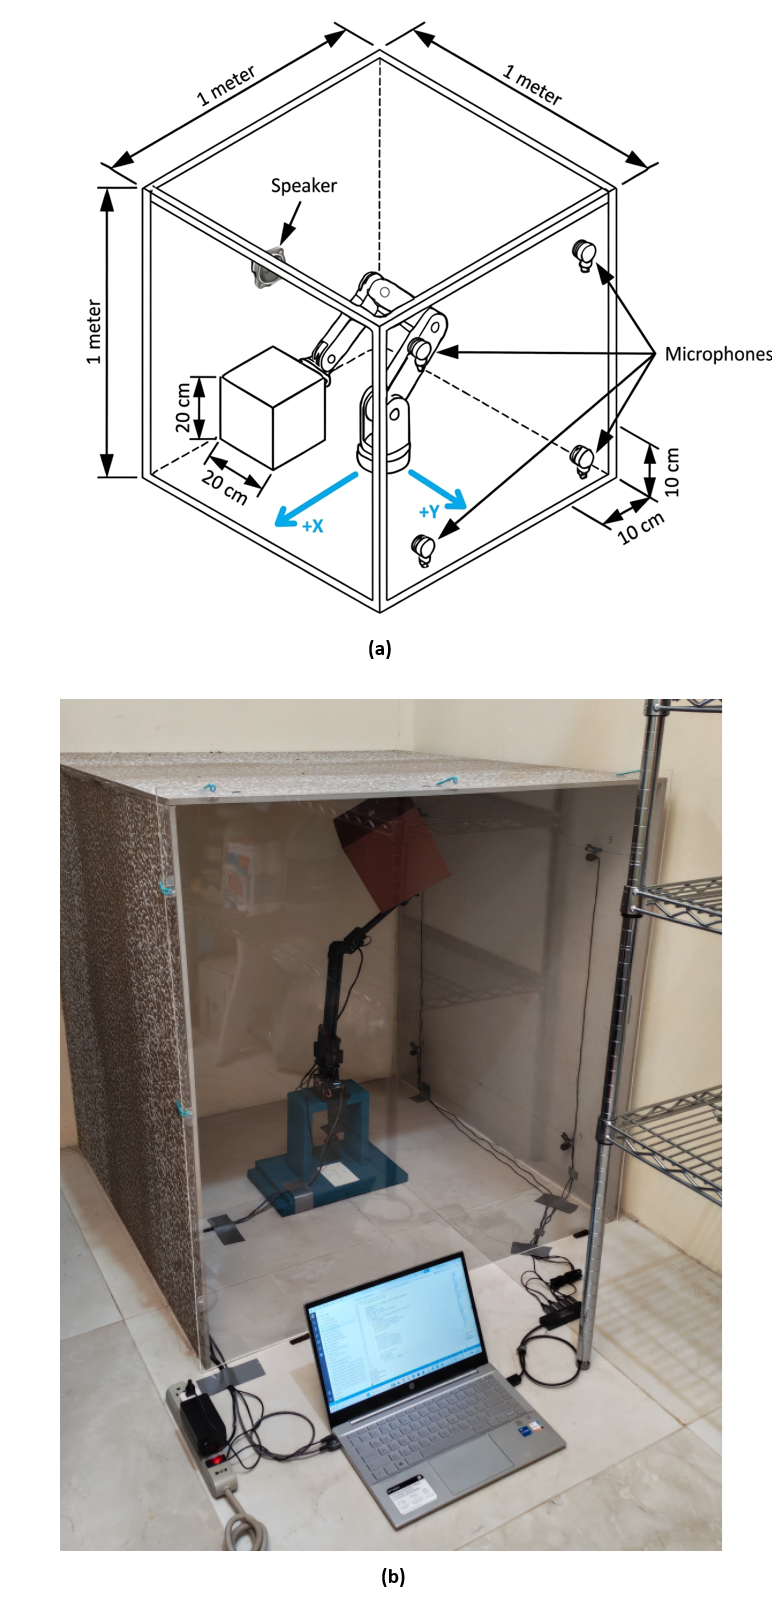
\includegraphics[height=15cm, width=8cm]{Measuretogether.png}
            \caption{Measure box: (a) Conceptual sketch for the acoustic measurement box, and (b) actual implementation for the data acquisition task.}
        \label{mesurementbox}                         
        \end{center}
\end{figure}



\subsection{The Audio-Location Dataset}

The dataset was collected through twenty‑six recording sessions. In each session, the robotic arm maintained a fixed angular value at its base and raised the cube to specific coordinates and orientations. The initial orientation of the cube was set with its sides parallel to the measurement box walls. The variables modified during each measurement were the cube’s location and orientation. For each location, nine different orientations were recorded. After completing these nine measurements, the robotic arm lowered the cube by decreasing its position along the Z axis, and the recording process was repeated for the new location. This procedure continued until the cube reached the bottom of the measurement box.

Audio from four channels was recorded. The acoustic signal was emitted four times, and the response was captured one microphone at a time. Each recording session consisted of 270 recordings, each containing four channels. A change of 10 degrees in the base of the robotic arm differentiated each recording session, producing a cylindrical envelope for the measurement area.

The coordinates of each measurement, obtained from the robotic arm, are shown in Fig. \ref{xyzlocations}. Each blue column in the three dimensions plot corresponds to the points in a recording session, and each point containts the nine orientations captured at that location. The total number of sessions was limited by the rotational constraint of the robotic arm’s base, which allowed only 270 degrees of angular movement in its base.

\begin{figure}[!htb]
        \begin{center}        
            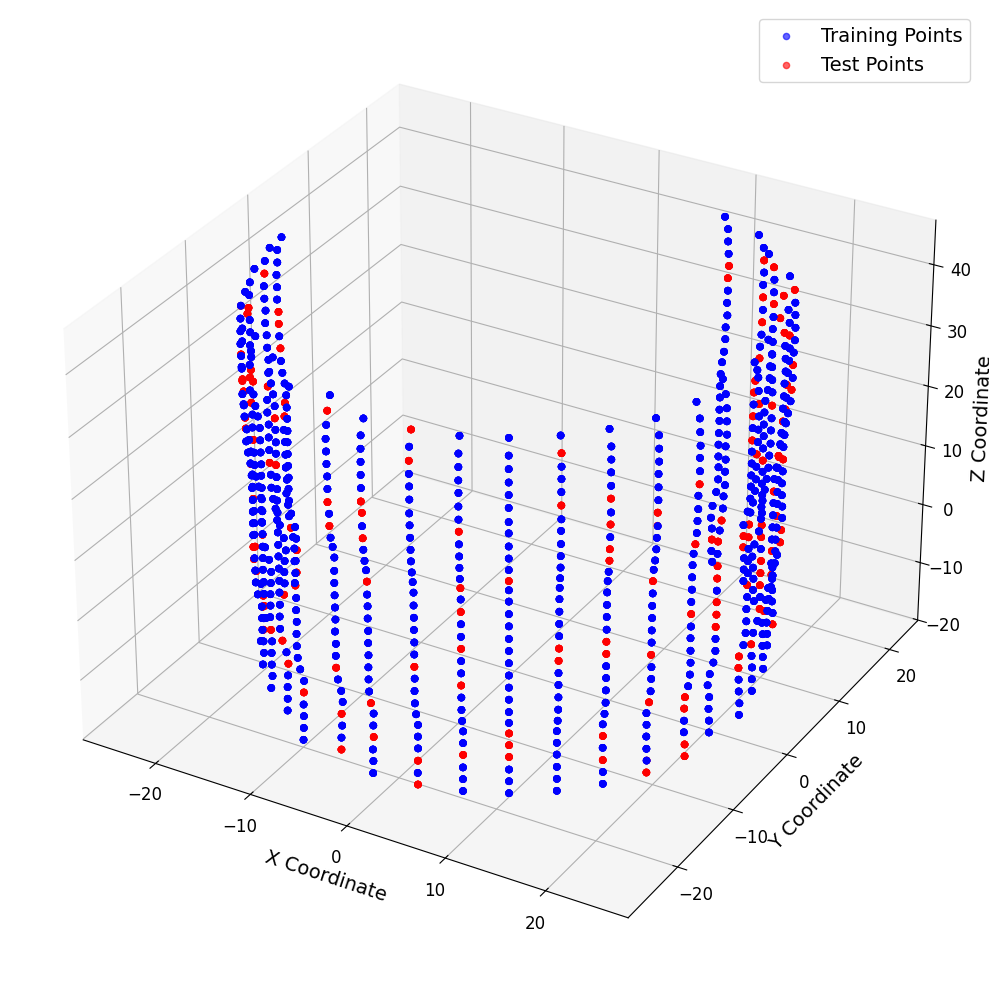
\includegraphics[height=9cm, width=9cm]{testpoints.png}
            \caption{Scatter plot of cube locations for each recording in the dataset, the blue columns represent the 26 sessions, and each point in the column represents the nine orientations captured at that location. The distribution of training and test points are pesentend in blue and red respectively.}
        \label{xyzlocations}                         
        \end{center}
\end{figure}

%##############################################################

The source audio signal was obtained by arbitrarily extracting a 0.3‑second segment from an acoustic melody. The spectrum of the signal has a bandwidth that reaches 10 kHz, with higher‑magnitude components concentrated at low frequencies. Before reproducing the source signal, the recording process is initialized by opening the capture window for one second. This procedure is repeated four times, once for each microphone. After completing the four recordings, the cube is moved to a new orientation until it complete the nine possible and after this it moves to a new location.

Due to the temporal unpredictability in the recording start time caused by the OS process scheduler, the signals from the four channels are aligned by exploiting the fact that the distance from the source to each microphone is identical. Therefore, the magnitude of the direct sound can be used as an alignment reference for the signals.

Second, a signal‑integrity validation is performed to divide each recording into its main body and tail (reverberation segment). From the main segment, the signal power is computed, and from the tail, its duration is extracted. Signals whose power and tail length fall within predefined limits are considered valid and included in the dataset.


To employ a CNN to train on the dataset a Log-Mel transformation is perform to the audio signals in order to obtain spectograms that ca be use as input for the network. Resulting in four log-mel spectogram images of 570x370 pixes per location-orientation as show in Figure \ref{spectogram4ch}. 

\begin{figure}[!htb]
        \begin{center}        
            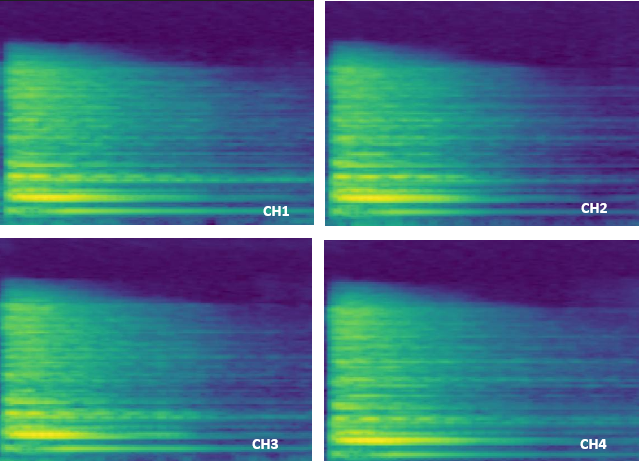
\includegraphics[height=5cm, width=8.5cm]{4channelSpec.png}
            \caption{Log-Mel spectograms correspondig of the four channels of signals captured at session 1, location X=22.8, Y=-0.94 , Z=-9.43 and orientation 50 degrees.}
        \label{spectogram4ch}                         
        \end{center}
\end{figure}



\subsection{CNN Architecture for Estimation}

The model architecture selected for the task of classifying and estimating the location–orientation of the cube inside the measure box was the ResNet‑18 network, chosen for its robustness, simplicity, and suitability for inference in resource‑constrained environments \cite{Resnetwhy}. Two modifications were applied to the standard network structure. First, the input layer was extended to accept a stack of four RGB images, one corresponding to each channel. Second, for the regression task, the softmax output layer was replaced with a single output feature using a sigmoid activation function.





The dataset collected is made up of 7020 samples, each sample composed of 4 images one for each channel. For training and validation it was split using an 80:20 ratio as show in Fig. \ref{xyzlocations} with the training and test points represented in blue and red respectively. Training was performed for 40 epochs for both the classification network and the regression network. The complete pipeline for the data processing is show in Figure \ref{method_flow}.


\begin{figure}[!htb]
        \begin{center}        
            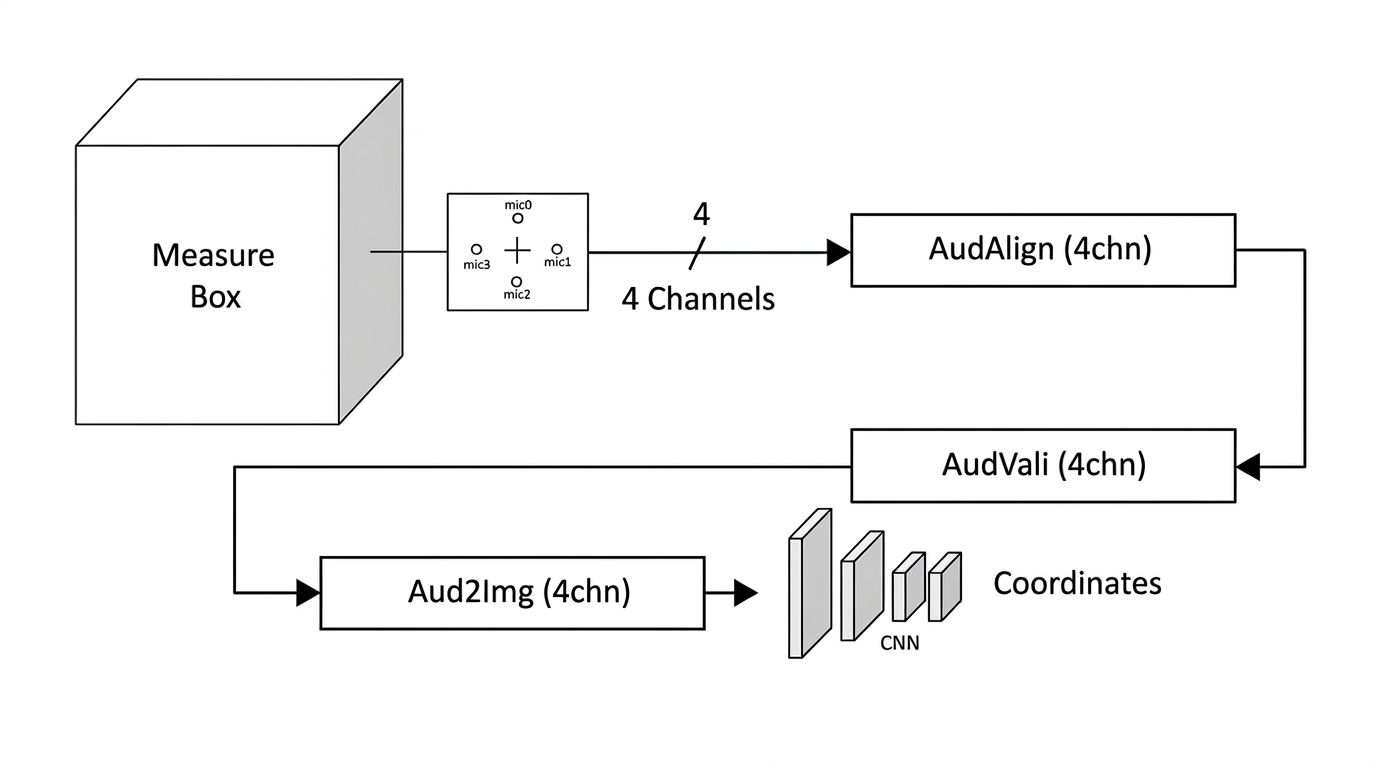
\includegraphics[height=6cm, width=9cm]{method2_improved.jpeg}
            \caption{Diagram of the audio data processing pipe for the estimator.}
        \label{method_flow}                         
        \end{center}
\end{figure}

\section{Results}

\subsection{Classification by Location and Orientation}

First, the capability of classifying the recordings in the database based on their location and orientation was explored. For the location classification task, the 26 distinct values of the session label were used to train the CNN. The objective of this experiment was to determine whether, after training, the network could correctly classify in which session each recording was perform. After training, the network achieved an accuracy of 99.3\% on the test set, producing only one misclassification out of the 1404 test samples.

For orientation classification, the dataset containing the 9 distinct label values and this information was used to train the network. The training procedure was identical to that of the location task, using 40 epochs. After training, the network achieved an accuracy of 27.07\% on the test set, exhibiting a high number of misclassification errors across the different orientations.


\subsection{Location Estimation}

To estimate the location along the X, Y, and Z coordinates, three independent networks were trained. In all the networks, the standard ResNet output layer was replaced with a single sigmoid function to enable training for regression instead of classification. Additionally, the loss function was changed from cross‑entropy which is used for classification to the MSE loss, since it operates on real‑valued outputs and computes the squared error between the predicted and actual values, making it suitable for regression.



The networks were trained for 40 epochs and subsequently evaluated using the test set. Figure~\ref{histograms} shows the resulting histograms and corresponding density curves for the estimation errors produced by each CNN for its respective coordinate.




From Fig.~\ref{histograms}, it can be observed that the error histograms for the X, Y and Z exhibit a symmetric distribution around zero presenting similarity to a normal distribution. The errors are concentrated betwent the range of -2cm to 2cm, with a few outliers extending beyond this range. The Z coordinate shows a wider spread of errors compared to the X and Y coordinates, indicating that the network has more difficulty accurately estimating the Z position of the cube in certain scenarios. 

\begin{figure}[H]
        \begin{center}        
            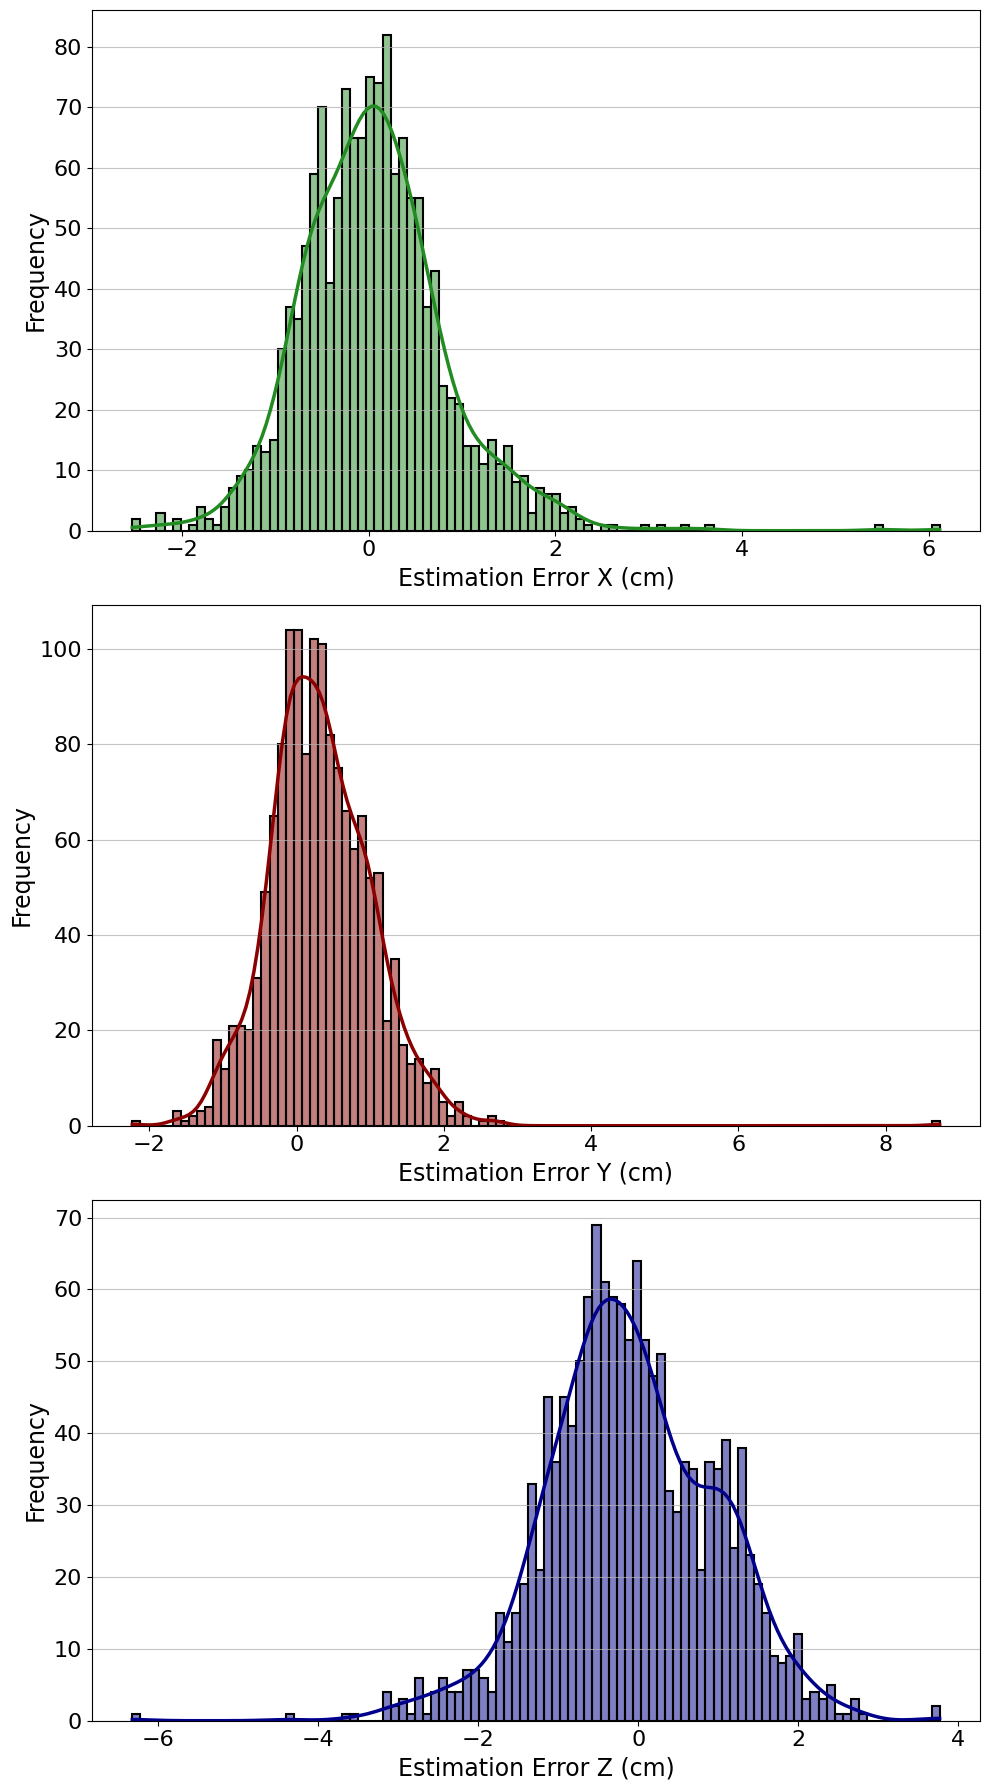
\includegraphics[height=15cm, width=8.5cm]{histograms_test_error.png}
            \caption{Histograms of the estimation errors for each coordinate with the test set after training.}
        \label{histograms}                         
        \end{center}
\end{figure}


The means and standard deviations for the histograms Fig.~\ref{histograms} are presented in Table~\ref{tab:meandesv}. The three coordinates exhibit mean values close to zero, indicating that the estimations are unbiased. The standard deviation for X and Y have a similar value near to 0.8cm, while the Z coordinate has a higher standard deviation of 1.05cm, indicating that the Z estimations are more dispersed. In all three cases the standard deviation is less than 2cm. Considering 
$2\sigma$ standard deviation as a metric of evaluation result in 95.44\% of the total estimations fall below 1.56cm of error in the X dimension, 1.42cm in the Y dimension and 2.11cm in the Z dimension. The table \ref{esterrorbyrange} shows the percentage of estimations that fall within different error ranges for each coordinate. The results indicate that the majority of estimations for all three coordinates fall within a range of $\pm2$cm, with the Y coordinate having the highest percentage of estimations within this range at 98.87\%, followed by X at 97.95\% and Z at 94.26\%. 

\begin{table}[!htb]
\centering
\begin{tabular}{lcc}
\hline
\textbf{Variable} & \textbf{Mean (cm)} & \textbf{Sample SD (cm)} \\
\hline
Error x & 0.0590 & 0.7869 \\
Error y & 0.3232 & 0.7112 \\
Error z & -0.1000 & 1.0577 \\
\hline
\end{tabular}
\caption{Mean and standard deviation for the three coordinates X,Y and Z}
\label{tab:meandesv}
\end{table}


The Fig.~\ref{boxplot} shows the boxplot for the distributions, it can be observed again that the error estimation is similar across the three coordinates
 when outliers are excluded from the analysis. For the three boxes the median is near to zero, the inter quartile range are comparable for X and Y, while Z has a larger inter quartile range. The whiskers in the graph represent the 1.5 times the inter quartile range and the outliers are represented as points beyond the whiskers.

 \begin{figure}[H]
        \begin{center}        
            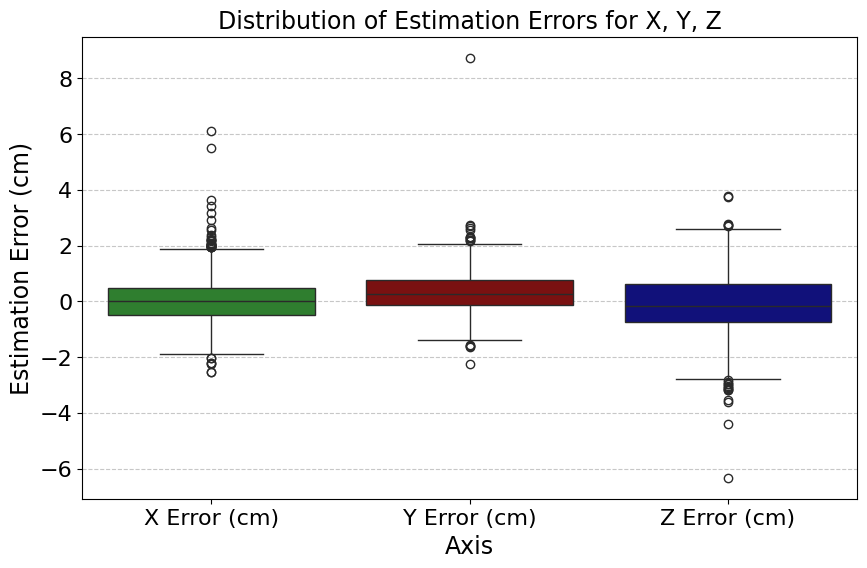
\includegraphics[height=5.5cm, width=8.5cm]{boxplot.png}
            \caption{Box-plot of estimation error for the three coordinates X, Y and Z}
        \label{boxplot}                         
        \end{center}
\end{figure}



To understand how the error relates to the cube’s location inside the box, Fig.~\ref{3derror} plots the absolute error as a function of the three spatial coordinates. to facilitate visualization, the error values are represented using a color scale, where blue indicates low error and red indicates high error. The outliers above the scale of 3 cm error are represented as points with a red color, indicating that they have a significantly higher error compared to the majority of the data. The plots show that the error is not uniformly distributed across the three dimensions but also is not evident that the error is concentrated in specific regions of the box. The error distribution appears to be more scattered, with some areas exhibiting slightly higher errors than others. There is no clear pattern or trend in the error distribution, suggesting that the network’s performance is relatively consistent across the different locations within the box. In the case of points near together in the test set, meaning that we had a low density of points in the training set for that area, the error  tends to be similar to the error of the points that are close to them, indicating that the network is able to generalize well in those regions.


\begin{figure}[H]
        \begin{center}        
            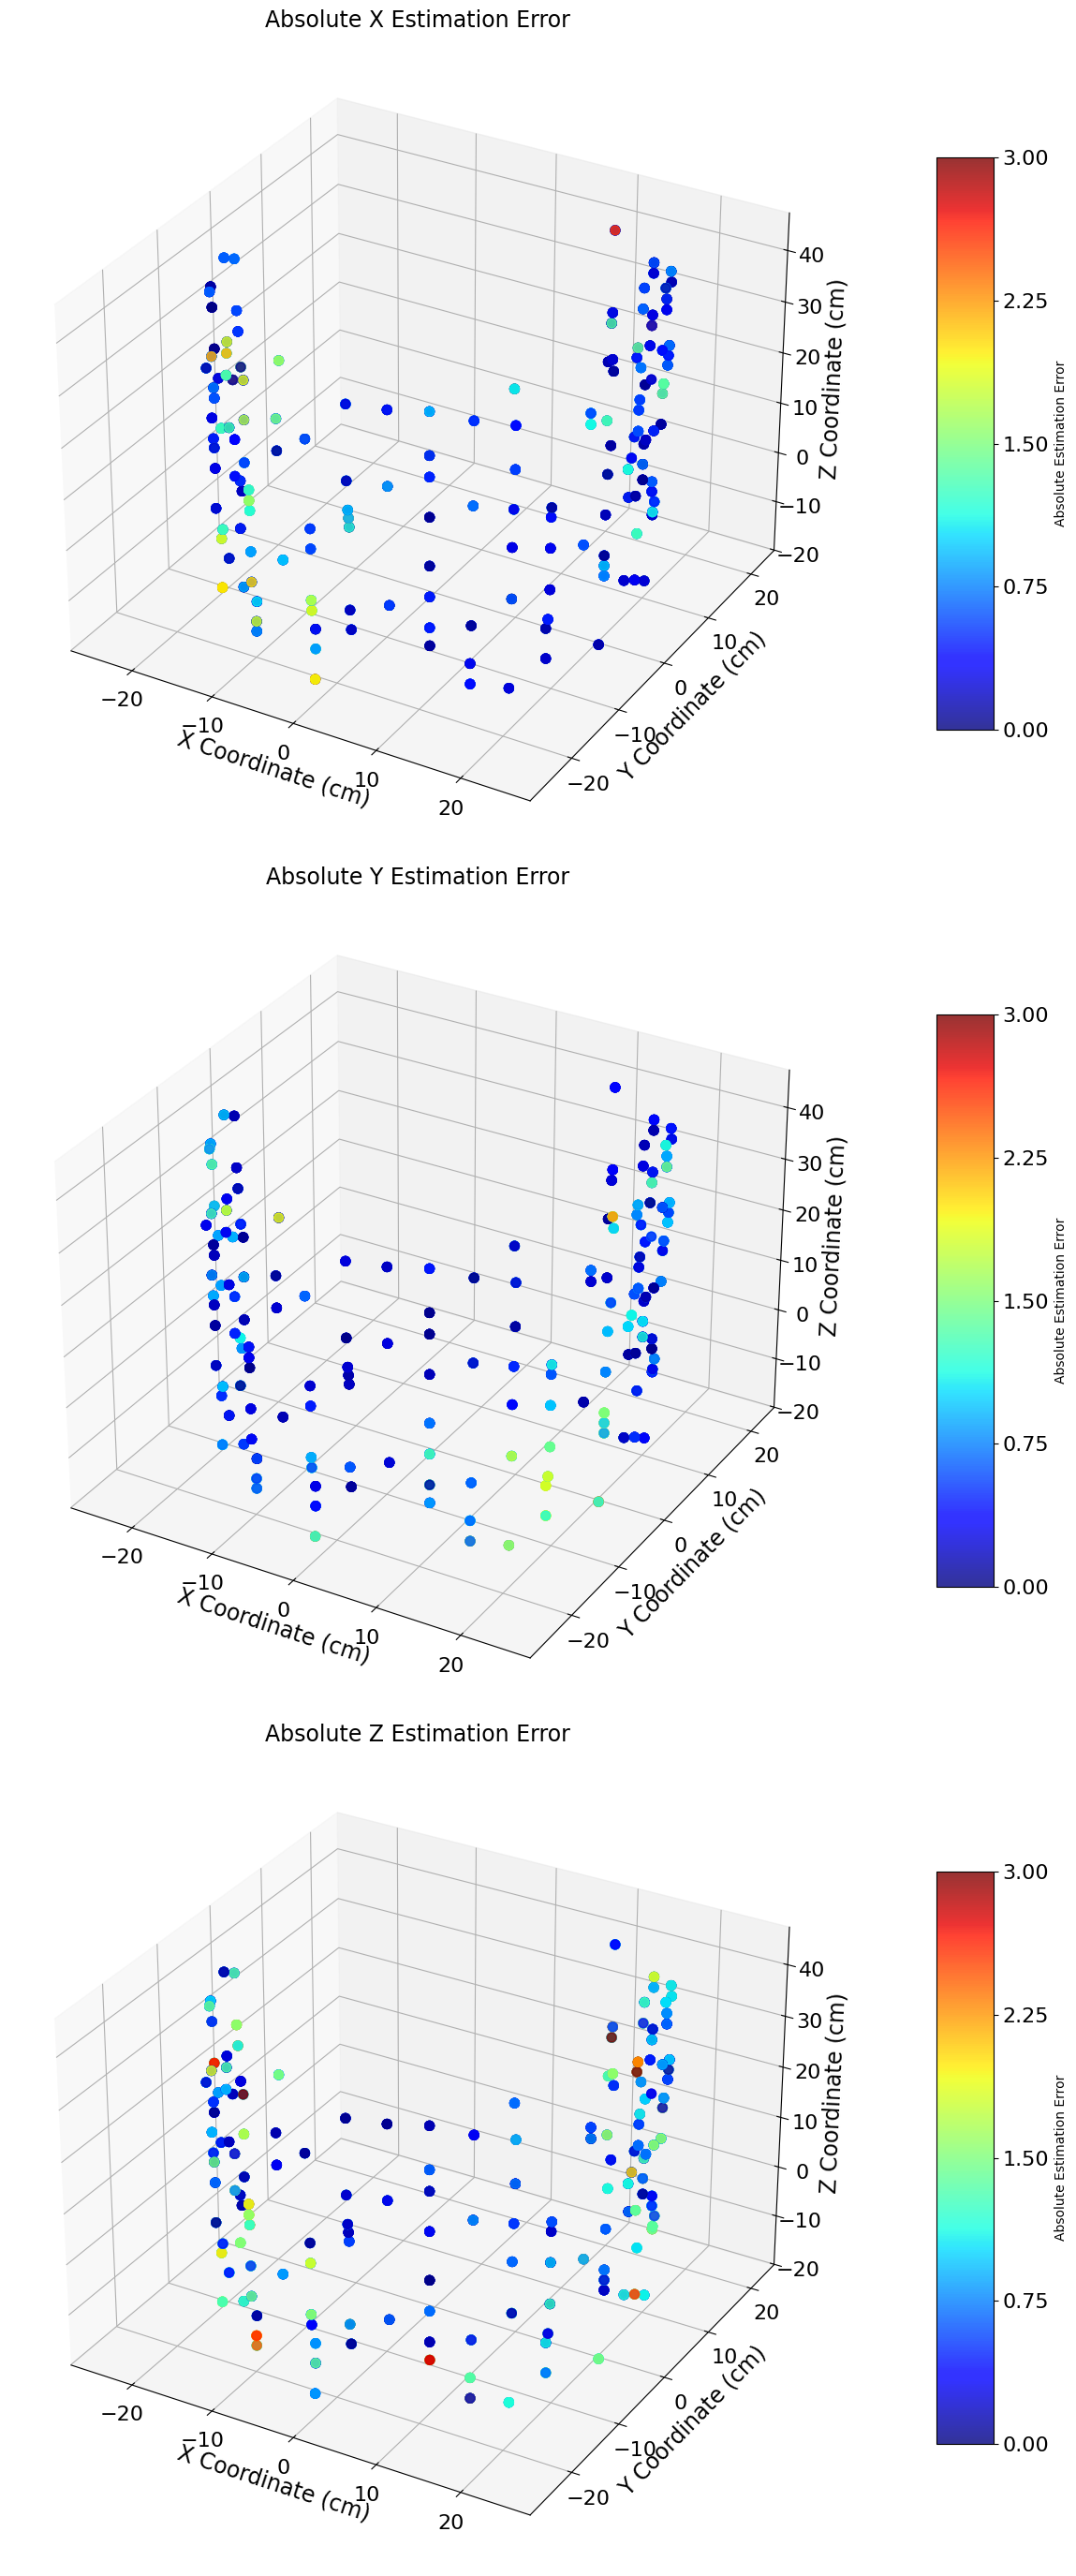
\includegraphics[height=16cm, width=9cm]{Estimation3D.png}
            \caption{Absolute value of the error estimation for the three networks as function of the three coordinates X, Y and Z}
        \label{3derror}                         
        \end{center}
\end{figure}



\begin{table}[h!]
\centering
\begin{tabular}{lccc}
\hline
\textbf{Error Range (cm)} & \textbf{Count X (\%)} & \textbf{ Count Y(\%)} & \textbf{Count Z(\%)} \\
\hline
(-1, 1) & 84.42 & 82.29 & 65.51 \\
(-2, 2) & 97.95 & 98.87 & 94.26 \\
(-3, 3) & 99.65 & 99.93 & 99.15 \\
(-4, 4) & 99.86 & 99.93 & 99.86 \\
\hline
\end{tabular}
\caption{Count of estimation error percentage by each error range}
\label{esterrorbyrange}
\end{table}



\begin{figure}[H]
        \begin{center}        
            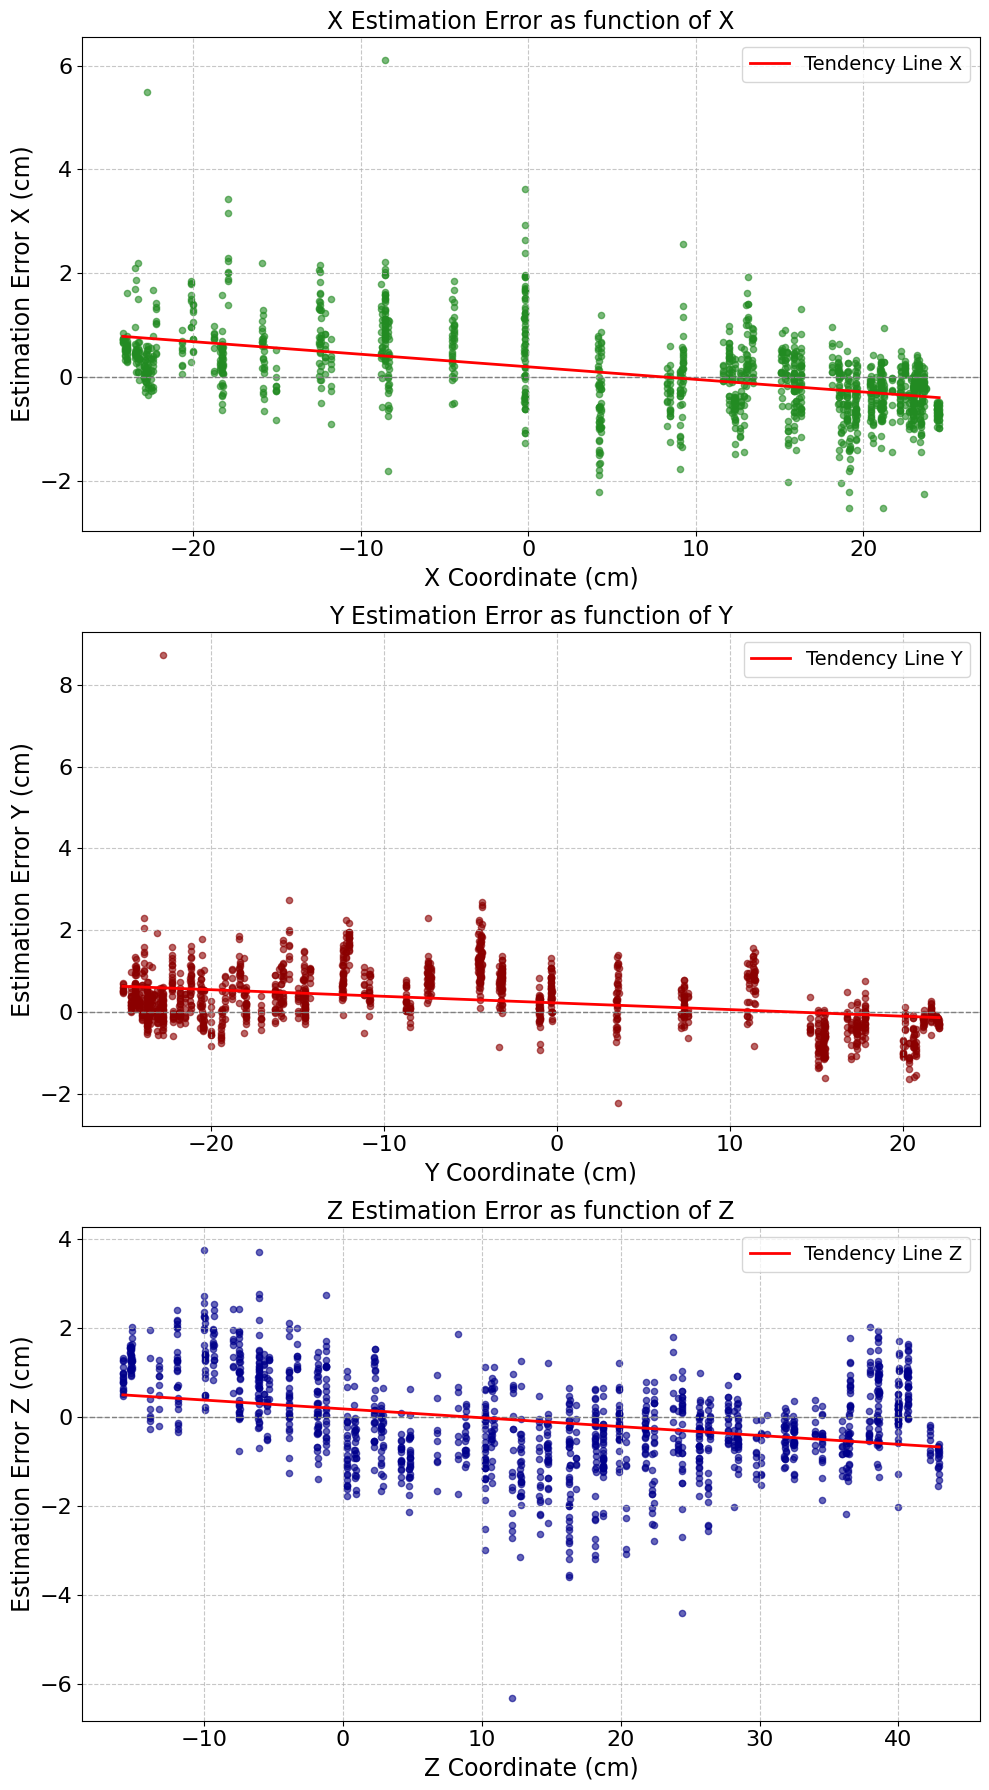
\includegraphics[height=14cm, width=8cm]{errorvscoordinates.png}
            \caption{Estimation errors along the three coordinates X, Y and Z as function of the corresponding coordinate value.}
        \label{XYZerror}                         
        \end{center}
\end{figure}

To extend and analyze more in detail the response of the networks along the coordinates, the network estimation error as a function  of individually the X, Y and Z coordinates is plotted in Fig.~\ref{XYZerror}. The estimation error was plotted as a function of each coordinate, with the other two remining coordinates having variations but not being the focus of the analysis. The plots include a tendency line in red obteined as the linear regression of the scatered points in the graph. The lines shows that the error moves from positive to negative when moving from negative to positive in the coordinates axis. Knowing that the error estimation is the diference betwen the predicted value and the real value, this means that the network tends to overestimate negative coordinates and underestimate positive coordinates. The tendency lines for the three coordinates evidence the same behaviour. Other aspects to highlight is that in X and Y the error is less in both extremes of the axis, this is due the fact that the movement of the cube for the data collection was circular in the plane X and Y causing that exist more points in the extremes of the axis, while in the middle of the axis there are less points and the error is higher. In contrast Z was uniformly sampled along the axis, with similar density of points along the axis.



%%\subsection{Limitations}


\section{Conclusion and Future Work}

The experiments presented in this work demonstrate that, from the acoustic response recorded by an array of microphones, it is possible to locate an object within a confined, reduced space. Regarding the classification task based on the acoustic response, the results show that identifying whether an object is positioned within a particular region ofthe measurement box is a trivial task for a CNN trained on Log‑Mel spectrograms. In contrast,the network exhibited poor performance when attempting to classifythe specific orientation ofthe cube.

For the task of estimating the cube’s position in a Cartesian coordinate system, the results indicate that the estimator exhibits a similar overall behavior across the three coordinates, although the estimation error varies slightly along each axis, the results present errors fitting the normal distribution. Among the three coordinates, the estimation of Y achieved the highest success rate, followed by X, and finally Z. The estimators for the three coordinates were capable of determining the cube’s position in most cases within an error range of $\pm2$cm.

This work did not consider the individual contribution of each channel; therefore, future research should explore the influence of each microphone on the overall estimation performance. Additionally, the histograms for the test set revealed a pattern suggesting two distinct distributions for X and Y. This observation, together with the axis‑wise error plots showing two different behaviors, suggests that dividing the estimation process for each axis into two separate regions may help reduce the error range. Finally, further investigation is needed to understand the impact of cube locations associated with problematic Z estimations and how these positions affect the estimation of the other coordinates.

\nocite{*}

\bibliographystyle{IEEEtran}

\bibliography{bibli}{}

%\appendix{}



\end{document}


